\documentclass{bioinfo}
\copyrightyear{2011}
\pubyear{2011}

\usepackage{multirow}
\newcommand{\Gossamer}{\textit{Gossamer}{}}
\newcommand{\Xenome}{\textit{Xenome}{}}
\newcommand{\Tophat}{\textit{Tophat}{}}
\newcommand{\rhomer}{$\rho$-mer{}}
\newcommand{\rhomers}{$\rho$-mers{}}
\newcommand{\kmer}{$k$-mer{}}
\newcommand{\kmers}{$k$-mers{}}
\newcommand{\fpkm}{\ensuremath{\hbox{\textit{FPKM}}}{}}
\newcommand{\dna}[1]{\textsc{#1}}

\newtheorem{defn}{Definition}

\begin{document}
\firstpage{1}

\title[Xenome]{Xenome --- A Tool for Classifying Reads from Xenograft Samples}
\author[Conway \textit{et~al}]{
Thomas Conway$^{1}$\footnote{to whom correspondence should be addressed}\ , Jeremy Wazny,$^1$ Andrew Bromage,$^1$  
 Martin Tymms,$^2$ Dhanya Sooraj,$^2$ Elizabeth D. Williams$^2$
and Bryan Beresford-Smith$^1$}
\address{$^1$NICTA Victoria Research Laboratory, Department of Computer Science and Software Engineering, The University of Melbourne, Parkville, Australia\\
$^2$Monash Institute of Medical Research, Monash University, Clayton, Australia\\}


\history{Received on XXXXX; revised on XXXXX; accepted on XXXXX}

\editor{Associate Editor: XXXXXXX}


\maketitle

\begin{abstract}

\section{Motivation:}
Shotgun sequence read data derived from xenograft material contains a
mixture of reads arising from the host and reads arising from the graft.
Classifying the read mixture to separate the two allows for more precise analysis
to be performed.

\section{Results:}
We present a technique, with an associated tool \Xenome, which
performs fast, accurate and specific classification of xenograft derived
sequence read data. We have evaluated it on RNA-Seq data from human,
mouse and human-in-mouse xenograft data sets.

\section{Availability:}
\Xenome\ is available for non-commercial use 
from \href{http://www.nicta.com.au/bioinformatics}{http://www.nicta.com.au/bioinformatics}

\section{Contact:} \href{tom.conway@nicta.com.au}{tom.conway@nicta.com.au}
\end{abstract}

\section{Introduction}

Xenograft models are an important tool for many areas of biomedical
research, including oncology, immunology and HIV pathology. A typical
scenario, drawn from oncology research, is that of a human prostate cancer
grown in an immunocompromised mouse model. Doing so allows researchers to investigate
aspects of the cancer that are not necessarily preserved in cell lines,
and it allows investigations into the interactions between the cancer and
the surrounding stromal tissue. The mouse may be biopsied or harvested
and samples of cancer and/or stroma collected at various time points during an experiment.

Difficulties arise, when sequencing the genome or transcriptome of the
samples because host (mouse) material (i.e. DNA/RNA) will inevitably
comingle with the graft (human) material.  If a sufficiently careful section
is taken, it has been generally assumed that the level
of host contamination is low enough that it may be ignored. This may be a
dangerous assumption, however, since the level of gene expression is
non-uniform. If the overall level of host contamination in a graft sample
is measured to be 10\% overall, it may still be the case for a given
gene that the host homologue accounts for most or all of the expression.

Contamination may be minimized by physical or biochemical techniques
such as conservative sectioning, cell sorting, or laser capture
micro-dissection, but these techniques can be a significant source of
technical bias, or in some cases may require infeasibly large amounts of
starting material. Further, in the case of transcriptomic investigation,
classifying host and graft \textit{in vitro} may fail to adequately
capture the interactions between them.

An alternative strategy is to sequence an acknowledged mixture of
host and graft, then use \textit{in silico} methods to classify
the individual sequence reads.  This is the approach discussed here.
We demonstrate a simple technique, based on an analysis of sequence reads
using \Tophat, and a more precise technique based on a \kmer\ 
decomposition of the host and graft reference sequences, \Xenome.
In both cases the primary goal of the analysis is to classify reads
into four classes: reads attributable to the \textit{host}, reads
attributable to the \textit{graft}, reads which could be attributed to
\textit{both}, and reads which are attributable to \textit{neither}.
To the best of our knowledge, there are no results in the literature examining
the classification of high throughput sequencing short reads from xenograft models.
The studies we know of are concerned with microarray expression profiles
or alternative methods for estimating the amount of host material or cell types in 
the samples. For example, \cite{Lin:2010p23155} investigate the use of species specific variation in gene length
and a multiplex PCR reaction to ascertain the relative amount of mouse and human DNA.
\cite{Wang:2010p29069} use microarray gene profiling data and \textit{in silico} techniques to estimate the 
quantity of various tissue components.
In \cite{Samuels:2010p29569} there is an analysis of a mouse xenograft model using microarray data.
They conclude that if there is more than 90\% human DNA then the expression profiles are not
unduly skewed. They also describe an experimental method for removing homologous genes based on 
cross-hybridization analysis of the probes. 
\cite{ding2010genome} use short read
sequencing to study a cancer genome and identify mutations/deletions.
They estimate tumour cellularity using pathological assessment, and
state that their xenograft is 90\% tumour cells. They also map NOD/SCID (mouse) genomic data
to human and mouse genomes, reporting 3.17\% and 95.85\% mapping rates
respectively and so apply no correction for the murine cells. 
We note that in the context of non-uniform RNA-Seq data ignoring the contribution
of the murine expression can lead to biases.

Tools such as \Tophat\ serve a different purpose than that of
\Xenome.  The former aligns reads to a reference, and we can use
those alignments for a variety of purposes, including the classification
task we present here. By contrast, \Xenome\ only performs the classification
task itself.
This is an important distinction, since an alignment must assign the
read to zero or more positions in the genome; the classification merely
has to decide if the read was more likely to arise from the genome than not.

For the remainder of the paper, we will assume, unless otherwise stated,
that sequence reads arise from RNA-Seq. However, the techniques we present
are applicable to genomic DNA sequences
(including ChIP-Seq and MeDIP-Seq) and also to other mixtures of DNA species.

\section{Methods}

Under the assumption that a graft sample has only a low level of host
material contamination, the simplest analysis is to use a regular
mapping-based RNA-Seq analysis tool, such as \Tophat\, and assume that
either the observed expression is dominated by the graft, which has
the greatest number of input cells, or that the homology between the
host species and graft species is such that reads arising from host
material will tend to map poorly, and the resultant inferred level of
gene expression will be negligible.

In some cases, these assumptions may be true, but in the case of human
cancer xenografts in mice, for example, the second assumption is false for many
transcripts, and a more precise technique is desirable.

Therefore, we have developed two techniques --- one based on the existing
RNA-Seq resequencing tool \Tophat\ \citep{tophat}, and one based
on $k$-mer decompositions of the host and graft references.
For genomic DNA, another resequencing/alignment tool could just as well be used.

\subsection{A \Tophat\ Based Method}
\label{sec:tophat}

A more precise analysis may be performed by using \Tophat\ \citep{tophat}
to analyze the reads. Firstly, \Tophat\ is used to process the read set with the graft genome as reference.
Secondly, \Tophat\ is used to process the read set with the host genome as reference.
Lastly, the accepted alignments from the \Tophat\ mappings are post-processed to  
partition the reads into four classes: 
 \textit{host}, \textit{graft},
\textit{both}, or \textit{neither}.
\Tophat\ provides mapping quality scores in its output, but they
only reflect whether or not the read mapped to multiple locations.
If the quality scores reflected a measure of certainty that the read
maps to the given location, a more sophisticated approach would be to
extend the classification to assign reads that map with high certainty
to one genome and low certainty to the other to the appropriate specific
class rather than \textit{both}. We do not pursue this further here.

An implementation of this method may be achieved easily
with \Tophat, \textit{SAMtools} \citep{Li:2009p29406} and some simple scripts. 
As will be apparent in
the results presented in Section~\ref{sec:results}, although very few
reads are misclassified (i.e. classified as \textit{host} instead of
\textit{graft}, or vice versa), a significant proportion of the reads,
even in a pure graft or pure host sample, fall in to the \textit{both}
class.
If these ambiguous reads were uniformly distributed in their origin
across the genome, this would have only a small impact, but as we will
elucidate in Section~\ref{sec:discussion}, the ambiguous reads are
non-uniformly distributed.
As a result, a significant number of genes cannot have their expression
unambiguously pinned to the host or the graft, though at least compared
to a single analysis, the set based analysis makes clear which reads
may be clearly associated with the host or the graft, and does not assume
that all gene expression in the sample is explained by the graft.

\subsection{ A \kmer\ Based Method}
\label{sec:xenome}

\begin{figure}
\begin{center}
\includegraphics[scale=0.7]{venn.pdf}
\end{center}
\caption{A Venn diagram showing the different classes that a given \kmer\ 
may belong to.  The marginal host (and marginal graft) partitions are
for those host (and graft) \kmers\ that are Hamming distance 1 from a
\kmer\ in the graft (and host) reference.}
\label{fig:venn}
\end{figure}

Our method proceeds in two phases: constructing a reference data
structure, then classifying reads with respect to that reference data
structure.  The reference structure is built from the sets of \kmers\ in
a pair of reference sequences, which we will refer to as the \textit{host}
and the \textit{graft}.

\subsubsection{Definitions}
\label{sec:xenome:defs}

Because in most sequencing protocols the reads are a mixture of forward and reverse complements
with respect to the reference sequence, we cannot assume the orientation of \kmers{} drawn from
reads will match the orientation of \kmers{} drawn from the reference. We could always consider both
orientations, but that would entail a lot of double handling of information, so instead we normalize
or \textit{canonicalize} \kmers.

\begin{defn}[\kmer{} canonicalization]

Consider a \kmer~$x$. We denote its reverse complement by $\bar{x}$.

A canonical \kmer~$\hat{x}$ is defined by a choice function $\mathcal{C}$
%whose value, given $x$ is 
giving a deterministic choice between $x$ and $\bar{x}$:
%$\mathcal{C}$ must have the property that
$$
    \forall x: \hat{x} = \mathcal{C}(x) = \mathcal{C}(\bar{x})
$$
\end{defn}

In principle, we can choose any such function: \textit{min} or \textit{max}
being obvious candidates, and the results of our method are identical for
all choices. In Section~\ref{sec:discussion} we will present
our specific choice which has important performance ramifications.

This definition can be extended to a set of \kmers\ $S$ in the obvious way:
$$
    \hat{S} = \left\{ \hat{x} : x \in S \right\}
$$

\begin{defn}[Marginal inclusion]
Consider a set of canonical \kmers~$\hat{S}$.  We say that a \kmer~$x$
is has \textit{marginal} membership of $\hat{S}$ if $\hat{x}$ does not
exist in $\hat{S}$, but has a Hamming distance 1 neighbor $y$ such that
$\hat{y}$ is a member of $\hat{S}$.

To aid our computation of marginal inclusion, we define the
function $\mathcal{M}$:
$$
\mathcal{M}(x, \hat{S}) =
        \{ \hat{y} : y \in \textit{Ham}_1(x) \} \cap \hat{S}
$$
where $\textit{Ham}_1(x)$ is the set of Hamming distance 1 neighbors
of $x$. Note that
$$
    \left\{ \hat{y} : y \in \textit{Ham}_1(x) \right\} =
    \left\{ \hat{y} : y \in \textit{Ham}_1(\bar{x}) \right\}
$$
\end{defn}

\subsubsection{Reference Construction}
\label{sec:ref}

For both host and graft reference sequences, we construct the set of
canonical \kmers\ ($\hat{H}$ and $\hat{G}$ respectively).  From these
we compute a complete set of canonical reference \kmers\ 
$\hat{S} = \hat{H} \cup \hat{G}$.
Note that $\forall x \in \hat{S}, x = \hat{x}$.

The sets of canonical \kmers\ tend to be large: with $k = 25$, there are
2.4~billion in the human genome, 2.1~billion in the mouse genome, and
4.5~billion in the union --- only 12~\textit{million} are shared.

A naive representation (2 bits per base, packed), would use 50 bits
per 25-mer, or about 26~GB. As discussed in our previous work
(\cite{ConwayBromage2011}), information theory gives a lower bound for the memory usage. For
a domain of $4^k$ possible \kmers, the minimum number of bits required
to represent a set of $n$ \kmers\  is
$$
    \log_2 {{4^k} \choose n}
$$
In the case of the union $\hat{S}$ above, this is about 10~GB, or less than half
what is required for the naive representation.  As also discussed in our
previous work, \textit{succinct} data structures have been developed to
give concrete representations that approach this theoretical lower bound.
The one we use, due to \cite{OkSa06}, works very well, requiring about 13~GB.

For each reference \kmer, we determine whether
it occurs in the host, the graft, both, or if it occurs in one and has
a marginal occurrence in the other. These classes are denoted \textbf{h}, \textbf{g},
\textbf{b} or \textbf{m}, respectively (see Figure~\ref{fig:venn}). 
More formally, we compute the
function $\mathcal{K}$ for each $\hat{x} \in \hat{S}$:
$$
    \mathcal{K}(\hat{x}) =
    \left\{
    \begin{array}{ll}
        \textbf{b} & \mbox{if } \hat{x} \in \hat{G} \wedge \hat{x} \in \hat{H} \\
        \textbf{g} & \mbox{if } \hat{x} \in \hat{G} \wedge \hat{x} \notin \hat{H}  \wedge ( \hat{H} \cap \mathcal{M}(\hat{x}, \hat{S}) = \emptyset ) \\
        \textbf{h} & \mbox{if } \hat{x} \notin \hat{G} \wedge \hat{x} \in \hat{H}  \wedge (\hat{G} \cap \mathcal{M}(\hat{x}, \hat{S}) = \emptyset )\\
        \textbf{m} & \mbox{if } \left( \hat{x} \in \hat{G} \wedge \hat{x} \notin \hat{H} \wedge ( \hat{H} \cap \mathcal{M}(\hat{x}, \hat{S}) \ne \emptyset ) \right) \\
                   & \mbox{ } \vee \left( \hat{x} \notin \hat{G} \wedge \hat{x} \in \hat{H} \wedge ( \hat{G} \cap \mathcal{M}(\hat{x}, \hat{S}) \ne \emptyset ) \right) \\
    \end{array}
    \right.
$$
$\mathcal{K}$ may
be extended to project not just \kmers\ to classes, but also a set of \kmers\ $\hat{Q}$ to a 
set of classes in the obvious way:
$$
    \mathcal{K}(\hat{Q}) = \{ \mathcal{K}(\hat{x}) : \hat{x} \in \hat{Q} \}
$$

These classes are precomputed and stored as a sequence of 2-bit values
corresponding to the \kmers\ in the succinctly store reference set.

The class $\textbf{m}$ denotes that the \kmer\ 
exists in~$\hat{H}$ and has \textit{marginal} membership of $\hat{G}$
or vice versa.  That is, they are \textit{marginally} distinctive,
in the sense that a single polymorphism or sequencing error may cause
a \kmer\ in that class to change from being marginally host to being
marginally graft.  Since the marginal set is symmetric (every marginal
host \kmer\ has a corresponding marginal graft \kmer, and vice versa),
and represents \kmers\ that are not very discriminating, we combine
both marginal sets into a single marginal set with the class $\textbf{m}$.

\subsubsection{Classification}
\label{sec:class}

Classification proceeds by taking each read $r$ and constructing the set
of canonical \kmers\ that may be derived from the read $\hat{Q}_r$. We
then map the set of \kmers\ to a set of classes by the function $\mathcal{K}$
described above.
\kmers\ that do not occur in the reference, $\hat{S}$, are ignored.
The \kmer\ classes that occur for a given read determine the classification
of the read as a whole according to the following function:
$$
C(\hat{Q}_r) =
\left\{
\begin{array}{ll}
    \textit{graft} & \mbox{if } \textbf{g} \in \mathcal{K}(\hat{Q}_r) \wedge \textbf{h} \notin \mathcal{K}(\hat{Q}_r) \\
    \textit{host} & \mbox{if } \textbf{g} \notin \mathcal{K}(\hat{Q}_r) \wedge \textbf{h} \in \mathcal{K}(\hat{Q}_r) \\
    \textit{ambiguous} & \mbox{if } \textbf{g} \in \mathcal{K}(\hat{Q}_r) \wedge \textbf{h} \in \mathcal{K}(\hat{Q}_r) \\
    \textit{both} & \mbox{if } \mathcal{K}(\hat{Q}_r) \cap \{ \textbf{g}, \textbf{h} \} = \emptyset \wedge \mathcal{K}(\hat{Q}_r) \ne \emptyset \\
    \textit{neither} & \mbox{if } \mathcal{K}(\hat{Q}_r) = \emptyset \\
\end{array}
\right.
$$
The read classes \textit{graft}
and \textit{host} denote cases where there is at least one \kmer\
which unambiguously comes from that \kmer\ class, and there are no
contradictory \kmers\ (i.e. unambiguously from the opposing reference).
The \textit{ambiguous} class corresponds to the case where there
are \kmers\ which appear to be contradictory --- unambiguously host,
and unambiguously graft. The \textit{both} class represents cases where
there are only \kmers\ which are either unambiguously common to both the
host and graft or \kmers\ which may belong to either if they contain a
single polymorphism or sequencing error. The last class, \textit{neither},
represents those cases where there were no matching \kmers.

\subsubsection{Implementation Concerns}

In Section~\ref{sec:xenome} we introduced an abstract canonicalization function
$\mathcal{C}$. The most commonly used concrete function is \textit{min}
(or \textit{max}) which selects the lexicographically/numerically smaller
of the \kmers~$x$ and~$\bar{x}$:
$$
    \mathcal{C}_{\textit{min}}(x) = \textit{min}(x, \bar{x})
$$

We use the following definition, assuming some reasonable hash function $f$:
$$
\mathcal{C}_{\textit{hash}}(x) =
\left\{
    \begin{array}{ll}
        x       & \mbox{if } \textit{f}(x) < \textit{f}(\bar{x}) \\
        \textit{min}(x,\bar{x}) & \mbox{if } \textit{f}(x) = \textit{f}(\bar{x}) \\
        \bar{x} & \mbox{if } \textit{f}(x) > \textit{f}(\bar{x})
    \end{array}
\right.
$$
Assuming $f$ is a reasonable hash function,
this definition effectively makes a random, but deterministic choice
between $x$ and $\bar{x}$.

We use this definition, rather than the more common lexicographic one,
because lexicographic canonicalization leads to the set of canonical
\kmers\ being non-uniformly distributed across the set of all possible
\kmers.

There are two ways in which a more uniform distribution of \kmers\ 
improves performance of \Xenome.
The first is that the succinct bitmap representation that we use
(due to \cite{OkSa06}) performs better on a uniform distribution of bits
(that is, a uniform distribution of \kmers).
The second is that it improves the performance of our intermediate
hash table, from which the succinct bitmap data structure is built.

The way the hash table is used is that as the input sequences
are read, they are decomposed into \kmers\ which are stored in the hash
table, which is of a fixed (controlled by a command line parameter) size.
When the hash table fills (that is, unresolvable collisions arise), it
is sorted and written out to disk. When all source \kmers\ have been
read, the sorted runs are merged and the main succinct bitmap is constructed.

The specific representation used is a succinct cuckoo hash table,
broadly similar to \cite{ArbitmanBackyardCuckoo}.
The succinct representation relies on the fact that the location of
the slot where a key $x$ (in this case, a \kmer) is stored
contains some of the information present in the key.

Consider an idealized hash table with load factor $1$ (i.e. the number
of values stored in the table equals the number of slots in the hash
table), with no collisions.
If the width of the hash table is $2^J$, then $J$ bits of
the key are implied by the slot chosen. For keys of $N$ bits, therefore,
the entries of the hash table need store only $N - J$ bits. The simplest
way this may be realized would be to just use $J$ bits of the key as
the slot number, and store the remainder in that slot, but of course,
this is likely to have an unacceptable number of collisions.

Instead, we use an invertible hash function (based on a single-stage
Feistel network, see~\citep{LubyRackoff88}) to turn a key $x$
into a slot number $s$ and
a stored component $v$ in such a way that given $s$ and $v$ we can
recover $x$ (assuming a hash function $f$):
$$
\begin{array}{ll}
    \mathcal{F}_f(x) & = \left\langle \left(x \mod 2^J\right) \oplus f(\frac{x}{2^J}), \frac{x}{2^J} \right\rangle \\
    \\
    \mathcal{F}^{-1}_{f}(\left\langle s, v \right\rangle) & = s \oplus f(v) + v2^J \\
\end{array}
$$

The size of the key data stored in the hash table is, then, $2^J (N-J)$ bits.
If $2^J \ll 2^N$, this is within
$\left(1 + o(1)\right) \log_2 {{2^N} \choose {2^J}}$ bits, and hence succinct.

(Of course, idealized hash tables are not possible if the set of
keys is not known in advance. Hence we use cuckoo hashing~\citep{Pagh04},
in which collisions are resolved (as far as possible) using multiple hash
functions.)

To make the sorting of keys more efficient, our hash function preserves
the~$N-J$ most significant bits of the keys, which are then stored
in the hash table (along with a few bits to determine which
hash function was used).
This means that we can perform an initial bucketing without inverting
the hash functions; the buckets can then be processed independently, using
multiple threads if required.

Now consider a set of random \kmers.
For hash-based canonicalization, given a good
hash function, there is an equal probability of observing any base
in the most significant position in $\hat{x}$. For lexicographic
canonicalization, there is a probability of $\frac{4}{10}$ that it is~\dna{a},
$\frac{3}{10}$ that it is~\dna{c}, $\frac{2}{10}$ that
it is~\dna{g}, and only $\frac{1}{10}$ that it is~\dna{t}. For a set
of $N$ random \kmers, the expected entropy at the most significant base
is $2.0$~bits and~$1.85$ bits respectively.

This matters, because hash functions are frequently vulnerable to poor
behavior in the presence of highly correlated sets of keys. In real,
biologically derived sets
of \kmers, the set of \kmers\ is non-random, so there is likely to
be less entropy to begin with, and therefore loss of entropy due to
canonicalization is exacerbated.
This is especially problematic in the case of the above family of
invertible hash functions, since it is precisely the most-significant
bits of the key which are passed to the underlying hash function~$f$.

The upshot of this is that $\mathcal{C}_{\textit{min}}$ leads to
highly correlated \kmers, which in turn lead to a high probability
of unresolvable collisions even when the hash table is nearly empty,
resulting in a large number of short runs.
Because the set of canonical \kmers\ that result from $\mathcal{C}_{\textit{hash}}$ are less correlated,
the hash table is unlikely to encounter unresolvable collisions until
it is almost full (80\%--85\% in practice).


\subsection{\Xenome\  --- Usage and Workflow}
\label{sec:usage}

To use the \texttt{xenome} tool, first it must be invoked to construct
the reference data structures. A typical invocation will give the
FASTA filenames for the host and graft genomes, a filename prefix for the
index files, and optionally, the amount of working RAM to use (in GB),
and the number of threads to use:
\begin{verbatim}
$ xenome index -M 24 -T 8 -P idx \
    -H mouse.fa -G human.fa
\end{verbatim}

This will run for some time --- on the human/mouse references, around
4--6 hours on an 8-core server. This need only be done once for a given
pair of references, and a given \kmer\ size. The \kmer\ size defaults to 25,
which seems to work well.

With the reference data structures built, read data may be segregated.
To make the output files easier to identify, command line flags can be
used to name the host and graft files. If paired data is being classified,
the \texttt{--pairs} flag should be given --- pairs are classified by computing
$\mathcal{K}(\hat{Q})$ over all the \kmers\ in the pair.

\begin{verbatim}
$ xenome classify -T 8 -P idx --pairs \
    --graft-name human --host-name mouse \
    --output-filename-prefix XYZ
    -i XYZ_1.fastq -i XYZ_2.fastq
\end{verbatim}

This yields the following set of files:

\begin{tabular}{ll}
\texttt{XYZ\_ambiguous\_1.fastq} &
\texttt{XYZ\_ambiguous\_2.fastq} \\
\texttt{XYZ\_both\_1.fastq} &
\texttt{XYZ\_both\_2.fastq} \\
\texttt{XYZ\_human\_1.fastq} &
\texttt{XYZ\_human\_2.fastq} \\
\texttt{XYZ\_mouse\_1.fastq} &
\texttt{XYZ\_mouse\_2.fastq} \\
\texttt{XYZ\_neither\_1.fastq} &
\texttt{XYZ\_neither\_2.fastq} \\
\end{tabular}

If the total size of the index files is larger than RAM, \texttt{xenome}
will perform poorly, but the flag \texttt{-M} can be supplied with the
maximum desired working set size, and the classification will be done in
multiple passes each using less memory.

On a single server with 8 AMD Opteron  cores running at 2 GHz and 
with 32~GB of RAM  \Xenome\  processes approximately $15,000$ read pairs per second.

Having classified the reads, typical usage would be to then run \Tophat\
and \textit{Cufflinks} to perform intron-aware gapped alignments and
compute gene expression. Instead of running \Tophat\ on all of the reads,
having separated the reads according to their origin, we can run it with
the human genome just against the human fraction of the reads, and against
the mouse genome on the mouse fraction of the reads.
It may well be desirable to combine the \textit{both} and \textit{ambiguous}
fractions with the human fraction to run against the human genome, and
also with the mouse fraction to run against the mouse genome. If this is done,
attention should be paid to homologous genes, since it is possible that
the human and mouse homologues may be represented by the same reads.
In some cases, the correct attribution of the gene expression may be apparent
from the nature of the experiment. For example, a sample from a human
prostate cancer grown in mouse may show ambiguous expression
in MYH genes which would be reasonably attributed to the stromal mouse tissue.

\section{Results}
\label{sec:results}

Our analysis examines two questions: whether or not it is
technically feasible to separate host and graft reads \textit{in silico};
and whether or not the fast technique we have proposed (\Xenome)
yields a worthwhile improvement over the mapping (\Tophat) based
technique.

\begin{figure}
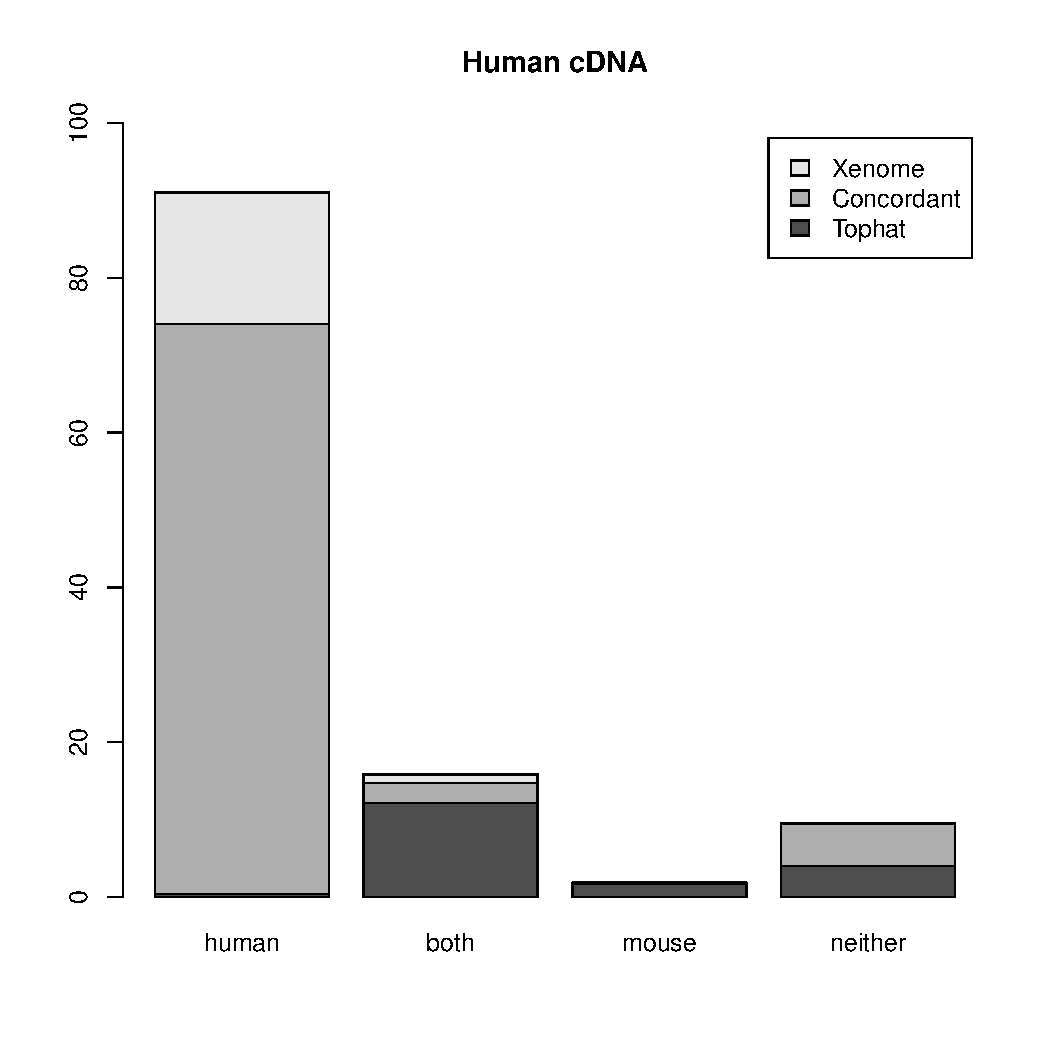
\includegraphics[scale=0.5]{human.pdf}
\caption{Summary of the results with Human cDNA. 
Each of the classes of reads is divided into those reads assigned to the class only by \Xenome\  (\Xenome), only by the \Tophat\ analysis (\Tophat) or by both \Xenome\ and the \Tophat\  analysis (Concordant).
}
\label{fig:human}
\end{figure}

\begin{figure}
\includegraphics[scale=0.5]{mouse.pdf}
\caption{Summary of the results with Murine cDNA.}
\label{fig:mouse}
\end{figure}

\begin{figure}
\includegraphics[scale=0.5]{bm18-26.pdf}
\caption{Summary of the results with BM18 xenograft cDNA.}
\label{fig:bm18-26}
\end{figure}

\begin{figure}
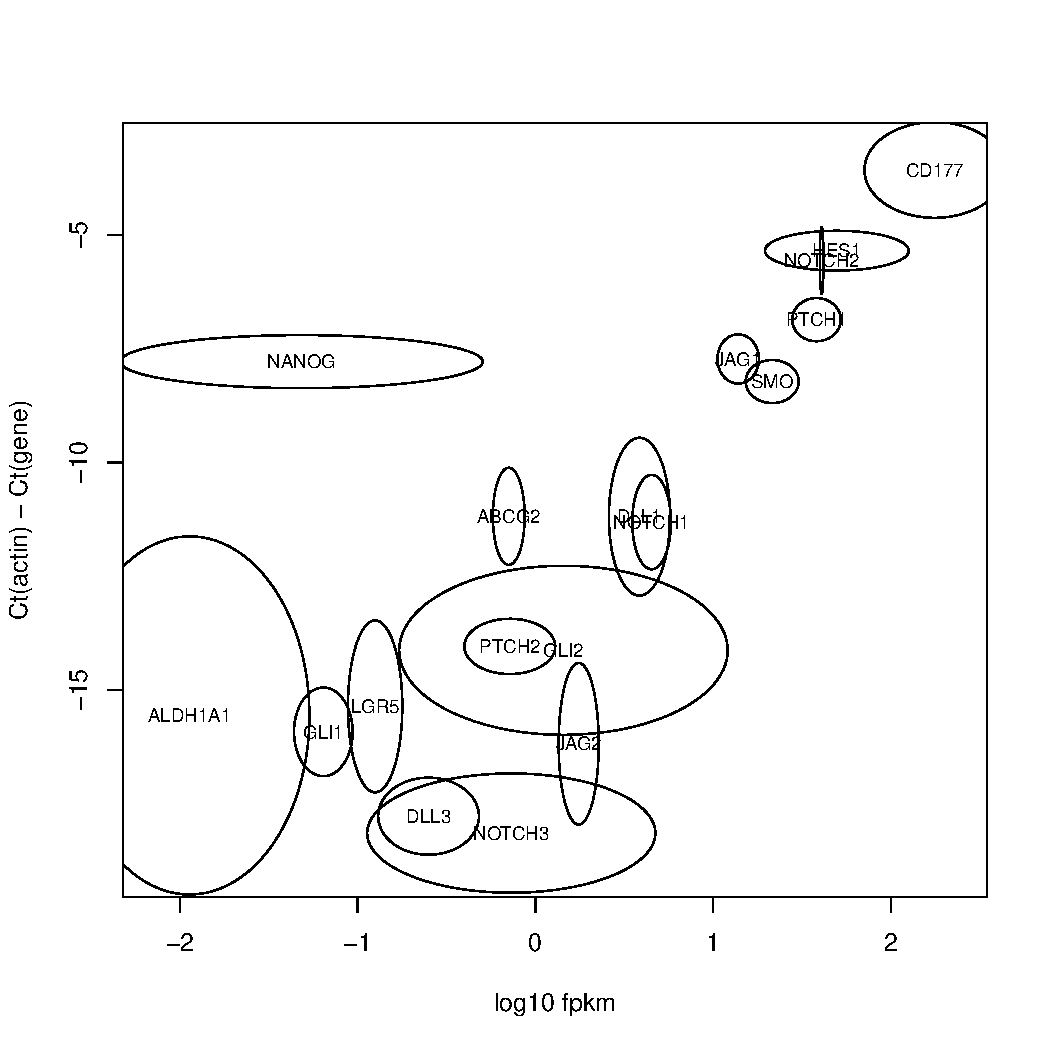
\includegraphics[scale=0.5]{validation.pdf}
\caption{Validation of the \textit{in silico} classification of xenograft RNA-Seq
data with qRT-PCR. The horizontal axis shows $\log_{10} \fpkm$ for the
\Xenome-derived gene expression for the 18 test genes. The vertical
axis shows the Ct value for each gene relative to the Ct of actin. There were
two RNA-Seq samples processed (biological replicates),
and 4 replicates of the qRT-PCR. For each gene, an ellipse is shown centered
on the mean $\log_{10} \fpkm$ in the x-axis, and on the mean relative
Ct in the y-axis. The horizontal and vertical radii show the variance in the
samples.
}
\label{fig:validation}
\end{figure}

In the first experiment,
we take a sample of human cDNA sequence data (SRR342886), and a sample
of mouse cDNA sequence data (SRR037689) and analyze them both with
\Tophat\ and \Xenome, and compare the results.  This allows
us to evaluate the degree to which sequences are misclassified (assigned
to \textit{human} rather than \textit{mouse} or vice versa), and the
specificity of the classification --- the proportion of sequences which
are not classified as \textit{both}.
The use of pure human or mouse cDNA gives an experiment
where the correct assignment of reads is known.

The second experiment runs the same analysis on
sequence data from a human prostate cancer xenograft growing in a mouse host (BM18, see \cite{MCCULLOCH:2005p18715}).
In this case, however, we not only classify
the reads, but use the \Tophat\ mappings to compute approximate
levels of gene expression (measured in fragments per thousand bases of
transcript per million mapped reads, or \fpkm\ (\cite{trapnell2010}) and
use human species specific quantitative RT-PCR (qRT-PCR) on
selected genes to validate the results.  In this instance, we have no
gold standard by which we can judge the results, but the qRT-PCR will
give some degree of validation, and known aspects of the biology of the
cancer can give some qualitative corroboration.

\Tophat\ uses a global analysis, combining the results of all the read mappings to
locate exons, junctions and so on. By contrast, \Xenome\ performs
pre-computation on the two reference genomes, then classifies each
read independently.
Therefore, for each of the three sets of reads, we ran \Tophat\ with
the human reference genome and again with the mouse reference
genome, then, as described in Section~\ref{sec:tophat}, the mappings
were post-processed to determine which reads belonged to each of the
four classes.  Each of the four partitions of the sets of reads was
then partitioned with \Xenome\ to allow us to easily determine
which reads were classified as the same by both procedures, and which were
classified differently.

Figures \ref{fig:human}, \ref{fig:mouse}, and \ref{fig:bm18-26}
summarize the results.  For the three samples, the proportion of reads
receiving the same classification were 82\%, 87\% and 84\% respectively.
As can be seen from the human and mouse only figures, both techniques
are accurate, in as much as they misclassify only a small proportion of
the reads (the worst case being the \Tophat-based analysis of
the human cDNA which misclassified 1.2\% of the reads --- all the other
analyses misclassified 0.2\% -- 0.3\%).  The main difference between
the \Tophat-based and \Xenome\ analyses is that the
latter yields better specificity --- the fraction of reads classed as
\textit{both} is significantly smaller in the \Xenome\ analysis.
To check for false positives for the human cDNA dataset we also used BLAT \citep{kent2002blat} to map the 1.1 million reads which
\Xenome\ classed as \textit{human} but which were not mapped to either genome by \Tophat.
Most of them were successfully mapped with high quality to the human reference by BLAT (about 90\%).
BLAT also mapped about 18\% of them, with very variable quality,  to the mouse reference.
This supports our confidence in the accuracy of the \Xenome\ algorithm.
From this we can conclude that the \textit{in silico} classification of
sequences is feasible and accurate.



The second experiment, using RNA-Seq data from a prostate cancer xenograft
into a mouse demonstrates that the classification works on a real mixture.
As described above, we performed the same process to partition the reads
into classes, then we used the refGene genome coordinates 
as calculated by \Tophat\  to assign
reads to genes, from which we computed an expression level using the
fragments per kilobase of transcript per million mapped reads formula
(\cite{trapnell2010}):
$$
    \fpkm = \frac{f \times 10^9}{zN}
$$
where $f$ is the number of fragments (reads, for single ended data, or
pairs for paired data), $z$ is the combined length of the exons of the
gene, and $N$ is the total number of mapped fragments.  Although this
quantification is peripheral to the technique we are presenting, we have
computed expression levels for the purposes of comparing with some qRT-PCR
data for the same biological data.  The qRT-PCR data were available for
18 genes: ABCG2, ALDH1A1, CD177, DLL1, DLL3, GLI1, GLI2, HES1, JAG1,
JAG2, LGR5, NANOG, NOTCH1, NOTCH2, NOTCH3, PTCH1, PTCH2, and SMO.
Figure~\ref{fig:validation} shows the $\log_{10} \fpkm$
versus the difference of the $Ct$ for each target gene and the $Ct$
for actin (which was used as a housekeeping gene).  With the exception of NANOG, the two methods correlate
reasonably well (the Pearson correlation coefficient is 0.80).  We have investigated the NANOG data, and cannot
explain the low \fpkm.
Whether this
is a sequencing issue or a biological variation in the mice is unknown, but
the low level of expression does not appear to be related to the behavior
of \Xenome\ or \Tophat.


\section{Discussion}
\label{sec:discussion}

\begin{figure}
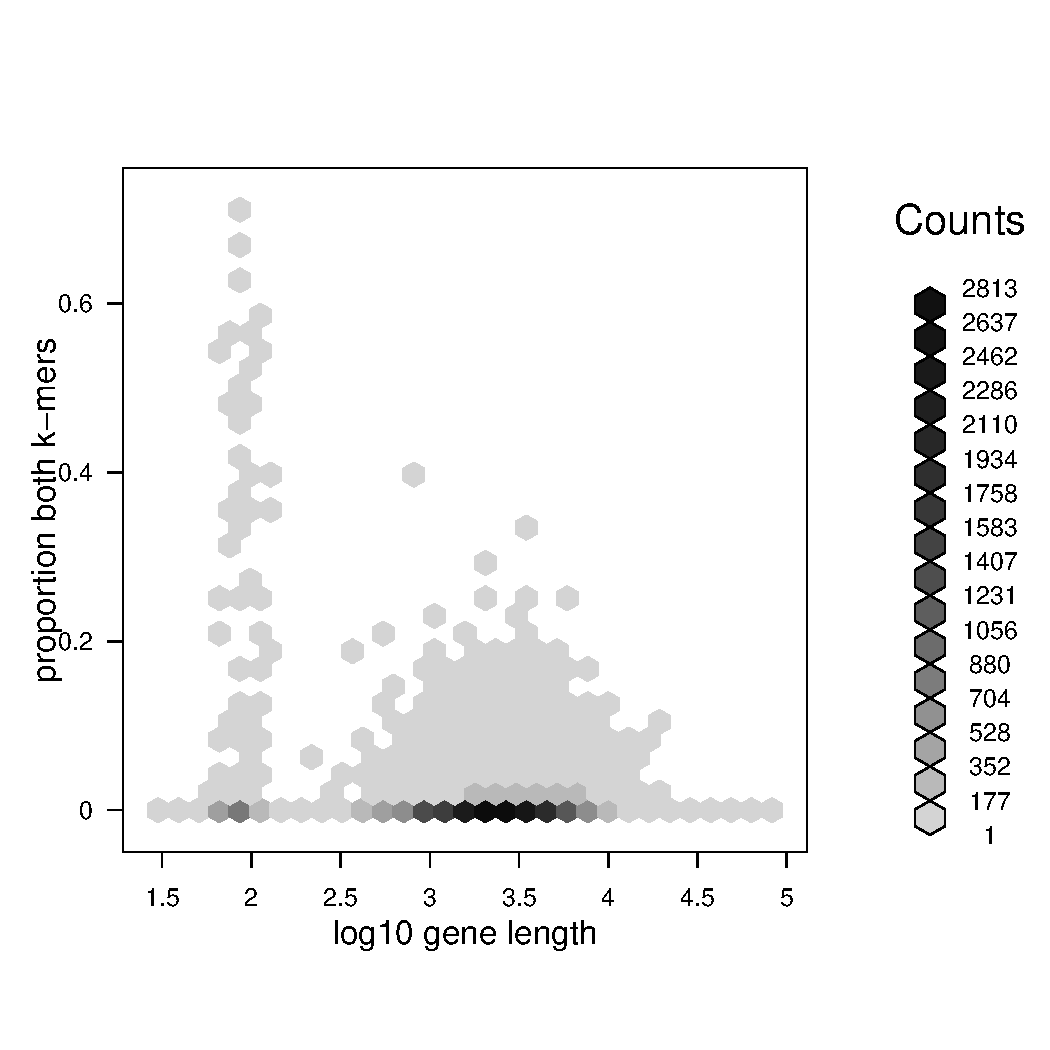
\includegraphics[scale=0.5]{both.pdf}
\caption{An \textit{in silico} analysis showing the degree of ambiguity in
HG19 refGene, according to the $k$-mer based analysis used by \Xenome. In
this analysis, $k = 25$.}
\label{fig:both}
\end{figure}

\begin{figure}
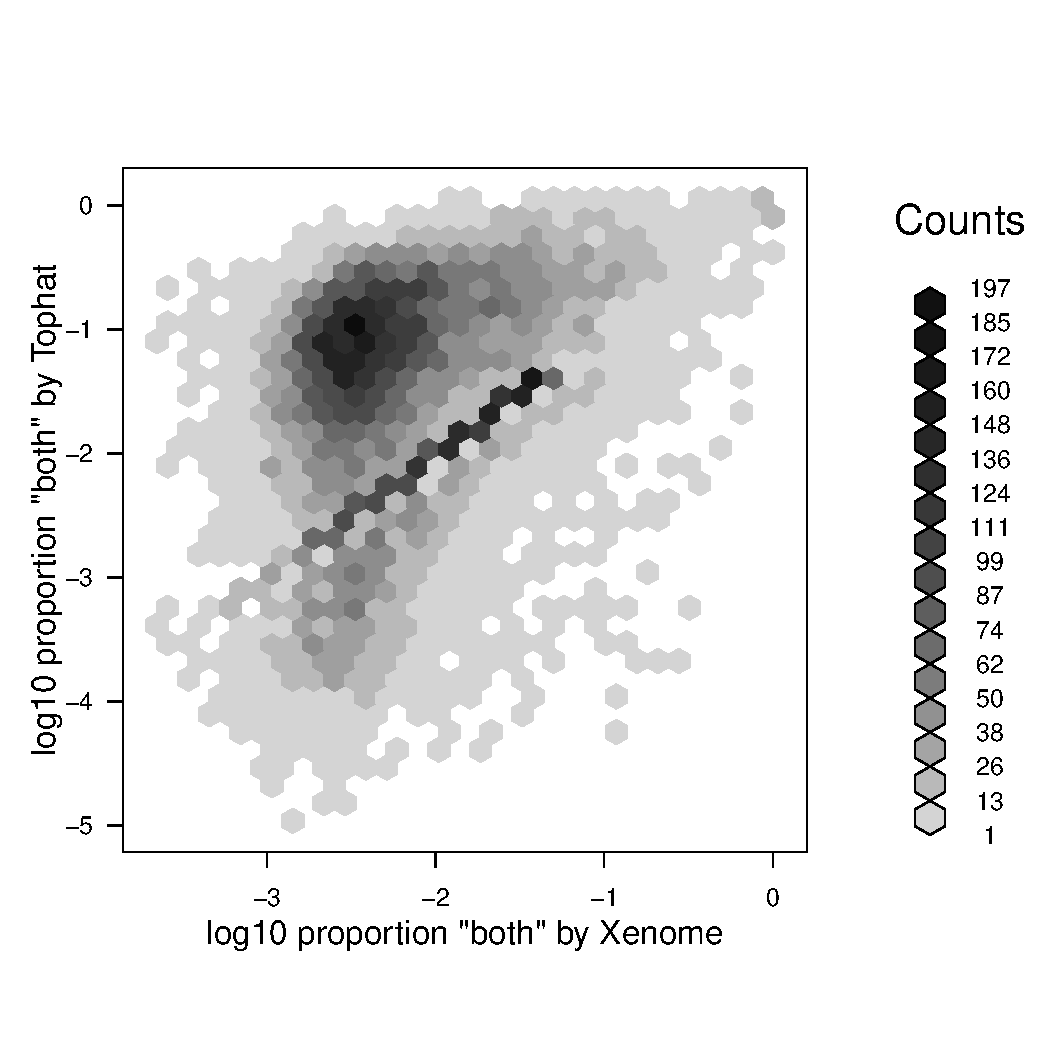
\includegraphics[scale=0.5]{rel-ambiguity.pdf}
\caption{A plot showing the distribution of human genes with respect to the
proportion of xenograft reads which are classed as \textit{both}
by the \Tophat\ based analysis and the \Xenome\ analysis.
The reads considered are only those mapped by \Tophat\ since \Xenome\
does not yield mappings, so cannot be used to assign reads to genes.
Only genes for which at least 20 reads mapped were considered.
The horizontal axis corresponds to the number of reads classified as \textit{both} or \textit{ambiguous} by \Xenome\ as a proportion of all the reads
that might possibly be human (i.e. \textit{both}, \textit{ambiguous}, or
\textit{human}).
The vertical axis corresponds to the number of reads classified as \textit{both}
by the \Tophat\ based analysis, once again, as a proportion of all the reads
that might possibly be human.
}
\label{fig:amb}
\end{figure}

We have presented a simple read classification method based on
\textit{Tophat}, and our refined classification approach, \textit{Xenome}.
\textit{Xenome} can be used to efficiently and effectively partition
the read set for subsequent processing by tools such as \Tophat.

What is not apparent from the results above is the
relative behaviour at the level of a single gene.
It should be expected that the distribution of ambiguously mapped reads
(classed as \textit{both}) should be non-uniform, since some genes in 
the two genomes are more highly conserved than others.

The first result we present in Figure~\ref{fig:both} on this point is
an \textit{in silico} analysis showing the proportion of each human
gene (ignoring introns) covered by $k$-mers that are not classed as
\textit{human}.  It is clear that the vast majority of genes contain few
or no $k$-mers that are not classed as \textit{human}.

The fraction of \kmers\ which are ambiguous gives a worst-case view
of how \Xenome\ might be expected to perform. In order for a read
to be classified as \textit{both}, all of its \kmers\ must be of the
\textit{both} class, or there must be at least one \kmer\  from each of the
two genomes (which happens less than 2\% of the time in the samples we
have tried).  Conversely, a single \textit{host} or \textit{graft} \kmer\
is sufficient to classify the read into the respective class. Therefore
for a read to be classified as \textit{both}, the reference must contain
a sufficiently long run of consecutive \kmers\ of class \textit{both}
and/or SNPs and sequencing errors must eliminate all the distinctively
\textit{host} or \textit{graft} \kmers.

The second result we report on this point, presented in Figure~\ref{fig:amb}
is the relative proportion of reads which are classified as \textit{both}
on a per-gene basis. What is evident in this figure is that although there
are many genes for which the proportion of \textit{both} reads is tightly
correlated between \Tophat\ and \Xenome, there are a large number of genes for which the \Tophat\ based
analysis has significantly more \textit{both} reads. There are 15,591 genes
for which there were at least 20 mapped reads in the BM18 xenograft sample.
Of these, there were 65 for which \Xenome\ assigned 
\textit{both} or \textit{ambiguous} to at least half the reads mapping to the gene;
there were 498 for which the \Tophat\ based analysis assigned \textit{both}
to at least half the reads mapped to the gene.
For the most highly conserved genes, there is not much that can be done
with this data directly --- further signal processing or other data would be required to determine the
relative expression in the host and graft.

While we have developed \Xenome\  with RNA-Seq on human/mouse xenografts in mind,
we anticipate it will be an effective tool for other similar mixtures.
For example, capturing the differential methylation around genes between
host and graft using MeDIP-Seq may shed light on the interraction between
the two.

The need for our technique is substantially motivated by the fact that
for a xenograft to be viable there must be very strong homology between
the host and graft organisms. This leads to a situation where there is a
high probability that a read may map to either genome, and it is this
problem that \Xenome\ specifically addresses. A side benefit is that the
classification is done independently for each read, and results in groups
of reads in each class; each group may then be processed independently
with further tools (such as \Tophat, \textit{Cufflinks} \citep{cufflinks},
or others). Given that many kinds of analysis require global processing of
the input data, being able to process a coherent subset of the data
can lead to a time/space gain. This benefit extends beyond the sphere
of xenografts. For example
there are situations where a parasite or pathogen cannot be cultured
independently (for example Chlamydia, and some fungi), so samples will
generally contain a mixture of host and pathogen. In some examples,
although the pathogen can be cultured independently, there are phenotypic
differences between organisms growing in culture and those growing in a
host. In both cases, there are benefits to being able to classify the
two groups of reads, even though straight mapping based approaches will
be less sensitive to cross-talk than xenograft data.

Precise alignment and alignment-free methods represent different points along
a spectrum of possible classification techniques.
Fundamentally, both rely on establishing homology between a
read and the host and/or graft references.
By substituting different algorithms for
establishing homology (e.g. various alignment algorithms, \kmer\ spectrum methods, etc),
different sensitivity and specificity might be achieved.

Although our current technique is built on simple set-based
classification, there is clearly scope to develop statistical models
which allow for a more subtle classification procedure.  These could,
for example, be based on the frequency of \kmers\ of different classes, giving
rise to the computation of the likelihood that a read
originated from either the host or graft genomes.  Indeed, if such
likelihoods were used from read alignments (\Tophat\ unfortunately
does not produce such scores), a unified model allowing either our
current \kmer\ based model or alignments could be used.

A further extension could take into consideration the established homology between genes in the
host and graft organisms. Where reads are ambiguous, non-ambiguous reads associated with the
same gene homologues could be used to help disambiguate the classification. EM based methods such as those described in \cite{Newkirk:2011cb, Chung:2011fv, Hormozdiari:2010jr}
would be a good basis for such an extension. We note however, that this would require significant
conceptual changes to \Xenome\ since it requires relatively more precise alignments.

It is instructive to consider a specific example of a gene where the \Tophat\ based and \Xenome\ analyses
are very different.
For the gene MYH3, in the human cDNA data set, there are 29 reads classed as \textit{human} by the \Tophat\
based analysis and 2,713 classed as \textit{human} by \Xenome. All the reads that are thus assigned by
\Xenome\ but not by the \Tophat\ based analysis were classed as \textit{both} by the latter. This is because
there is a high level of conservation in this gene between the two species, and the reads therefore
aligned to both.
Were \Tophat\ to yield meaningful alignment quality scores, a statistical approach of the kind hinted at
above may perform similarly to the \kmer\ based approach.


\section*{Acknowledgement}
%Text Text Text Text Text Text  Text Text.  \citealp{Boffelli03} might want to know about  text text text text

%\paragraph{Funding\textcolon} 
National ICT Australia (NICTA) is funded by the Australian Government's Department of Communications; 
Information Technology and the Arts;  
Australian Research Council through Backing Australia's Ability; 
ICT Centre of Excellence programs.

This project was supported in part by funding from the Prostate Cancer Foundation of Australia (EDW) and 
the Victorian Government's Operational Infrastructure Support Program. 
EDW is supported by an Australian NHMRC Career Development Award (\#519539).

\bibliographystyle{natbib}

%\bibliographystyle{achemnat}
%\bibliographystyle{plainnat}
%\bibliographystyle{abbrv}
%\bibliographystyle{bioinformatics}
%
%\bibliographystyle{plain}
%

\bibliography{paper}


% Nucleic Acids Res 34:1-9 (2006) Riley M, Abe T, Arnaud MB, Berlyn MK, Blattner FR, et al.
% "Escherichia coli K-12: a cooperatively developed annotation snapshot--2005." 

\end{document}
